\subsubsection{Batch approach: MapReduce}

\definition{MapReduce} is a \textbf{programming architecture} and an associated implementation for processing and generating big data sets with a parallel, distributed algorithm on a cluster.

\highspace
A MapReduce is composed of a \textbf{map procedure}, which performs filtering and sorting (such as sorting students by first name into queues, one queue for each name), and a \textbf{reduce method}, which performs a summary operation (such as counting the number of students in each queue, yielding name frequencies). The \dquotes{MapReduce System} (also called \dquotes{infrastructure} or \dquotes{framework}) orchestrates the processing by marshalling the distributed servers, running the various tasks in parallel, managing all communications and data transfers between the various parts of the system, and providing for redundancy and fault tolerance.

\begin{examplebox}[: an example of a batch approach using MapReduce]
    \begin{center}
        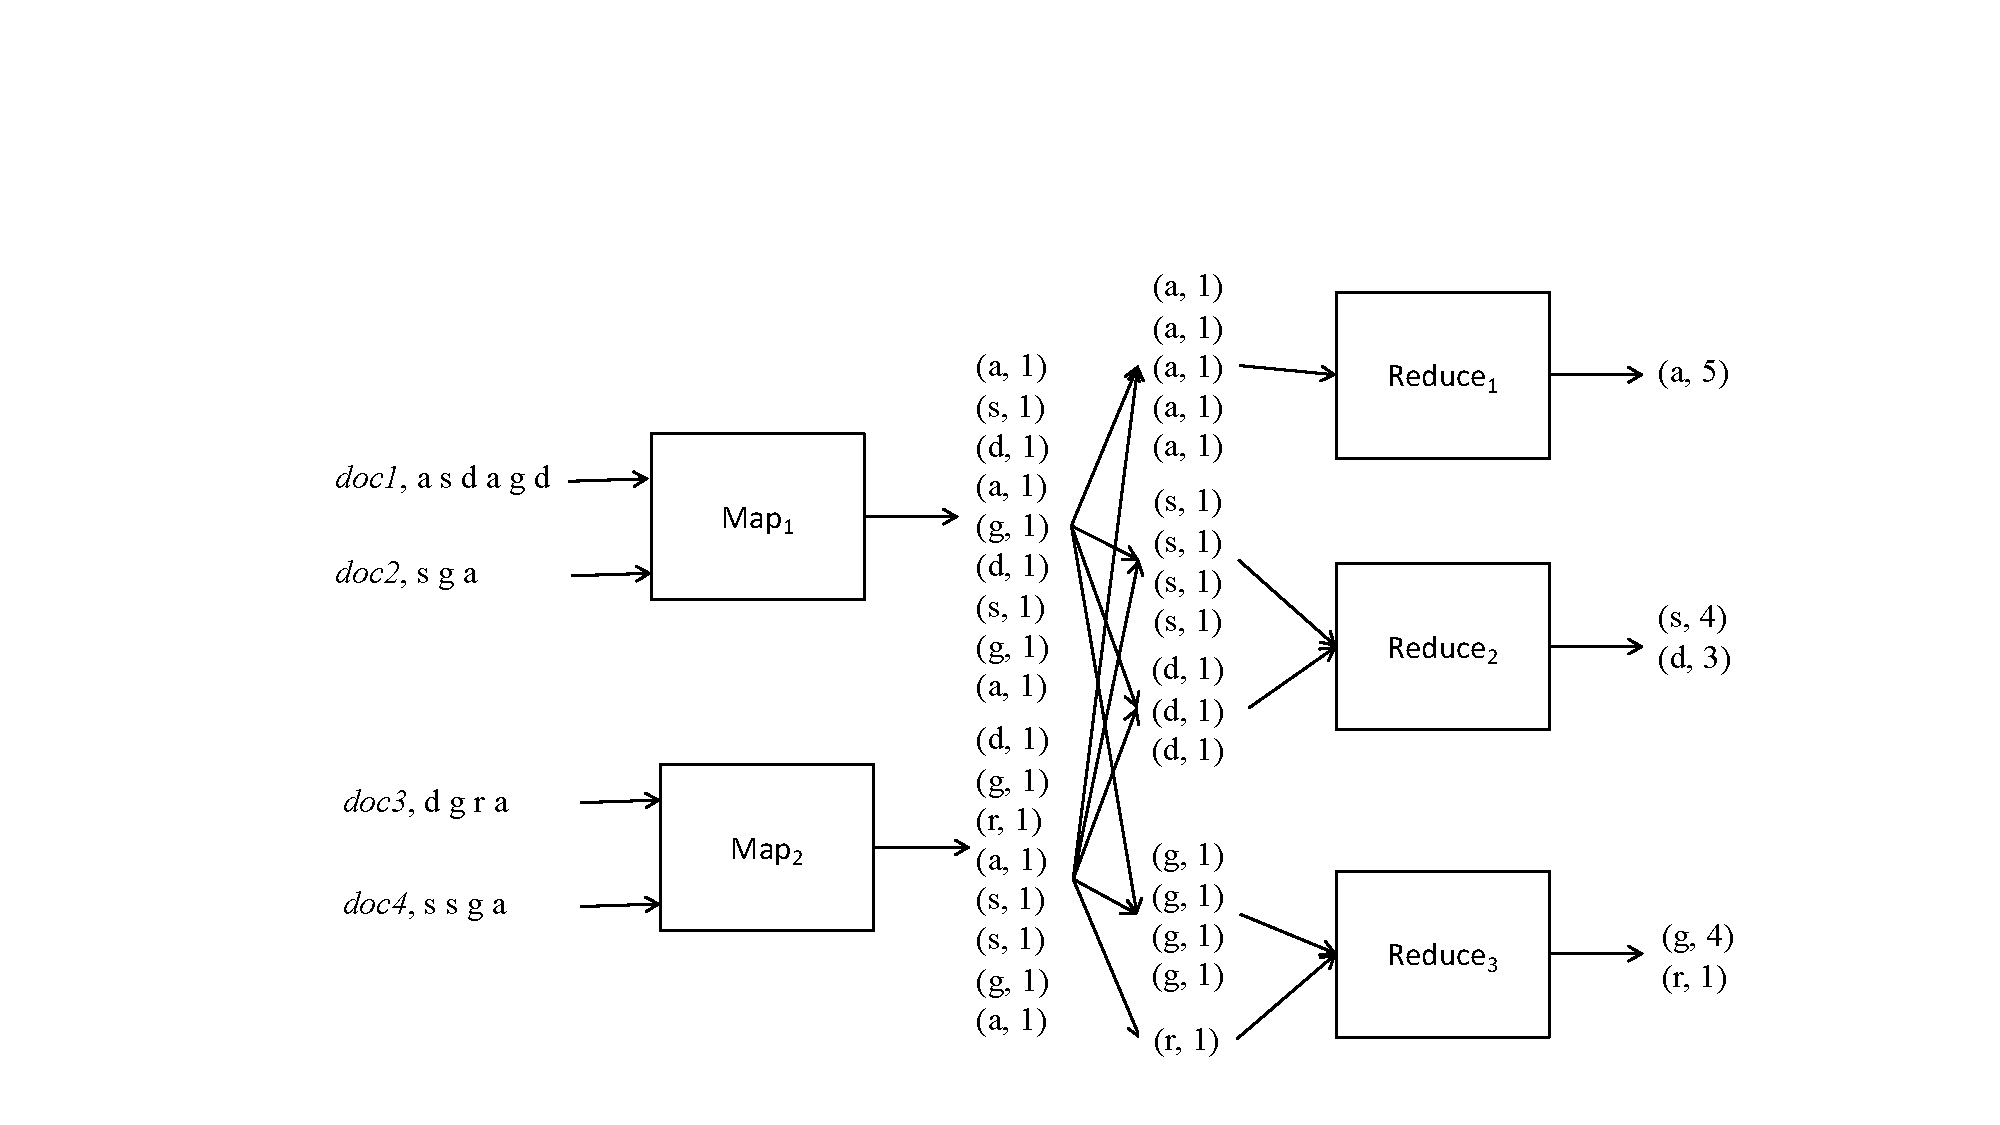
\includegraphics[width=\textwidth]{img/mapreduce-1.pdf}
    \end{center}
    The workflow is the following:
    \begin{enumerate}
        \item Read a set of input files and break it into records;
        
        \item Call the \texttt{map} function. It extracts a key and a value from each record (the assigned value is application-dependent);

        \item Sort all the key-value pairs by key;
        
        \item Call the reduce function. It iterates over the ordered sets of key-value pairs and combines the values (the combination logic is application-dependent)
    \end{enumerate}
\end{examplebox}

\newpage

\begin{figure}[!htp]
    \centering
    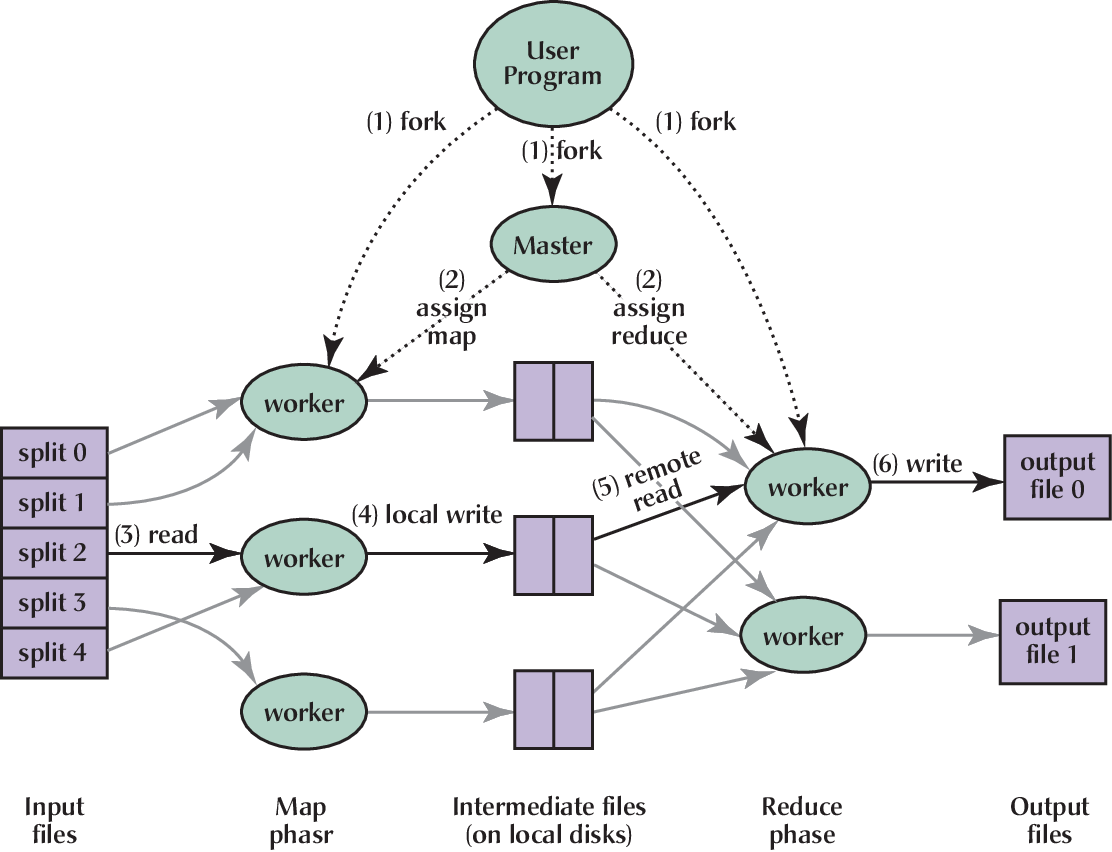
\includegraphics[width=\textwidth]{img/mapreduce-2.png}
    \caption{MapReduce architecture.}
\end{figure}

\begin{flushleft}
    \textcolor{Green3}{\textbf{\faIcon{check} Advantages}}
\end{flushleft}
\begin{itemize}
    \item Works well on commodity hardware.\footnote{Commodity hardware in computing is computers or components that are readily available, inexpensive and easily interchangeable with other commodity hardware. Almost all PCs use commodity hardware.}
\end{itemize}

\begin{flushleft}
    \textcolor{Red2}{\textbf{\faIcon{exclamation-triangle} Disadvantages}}
\end{flushleft}
\begin{itemize}
    \item Implementing a complex processing job is not simple (high level programming model have been built on top of it);

    \item Reducers have to wait until the preceding Mappers have concluded their job;

    \item Materialization of intermediate states can be overkilling;

    \item Sometimes it is not necessary to sort the results of mappers;

    \item New batch computation approaches supported by frameworks as Spark, Tez, Flink, etc.
\end{itemize}